\renewcommand{\NomeBloco}{Comparador}
\renewcommand{\NomePTab}{tab_\NomeBloco}
\renewcommand{\NomeSTab}{tab_\NomeBloco2}
\renewcommand{\NomePFig}{fig_\NomeBloco}
\renewcommand{\NomeSFig}{fig_\NomeBloco2}
\renewcommand{\NomeTTab}{tab_\NomeBloco3}

\section{\NomeBloco}

O bloco \NomeBloco{} tem a fun{\c c}\~ao de comparar dois sinais anal\'ogicos advindos nas entradas '+' (\emph{Vp}) e '-' (\emph{Vn}), e retornar \emph{VDD} caso Vp seja maior do que Vn, e \emph{GND} caso Vp seja menor ou igual a Vn.  O bloco apresenta as defini{\c c}\~oes de sinais de entrada e sa\'ida referidos na \autoref{\NomeSTab}.

\begin{table}[htbp]
\caption{Sinais do bloco \NomeBloco}
\label{\NomeSTab}
\centering
\begin{tabular}{ccl}

    \toprule
    Sinal & Tipo    & Descri{\c c}\~ao        \\
    \midrule \midrule
    Vp (+) & Entrada & Entrada positiva do Comparador\\
    \midrule
    Vn (-) & Entrada & Entrada negativa do Comparador\\
    \midrule
    Ibias & Entrada & Corrente de polariza{\c c}\~ao do Comparador\\
    \midrule
    Vo & sa\'ida & Sa\'ida do Comparador\\
    \bottomrule
\end{tabular}
\legend{Fonte: Produzido pelo autor}
\end{table}

O circuito projetado para o bloco \'e demonstrado na \autoref{\NomePFig}.

\begin{figure}[htb]
 \label{\NomePFig}
 \centering
    \centering
    \caption{Circuito CMOS projetado para o bloco \NomeBloco} 
    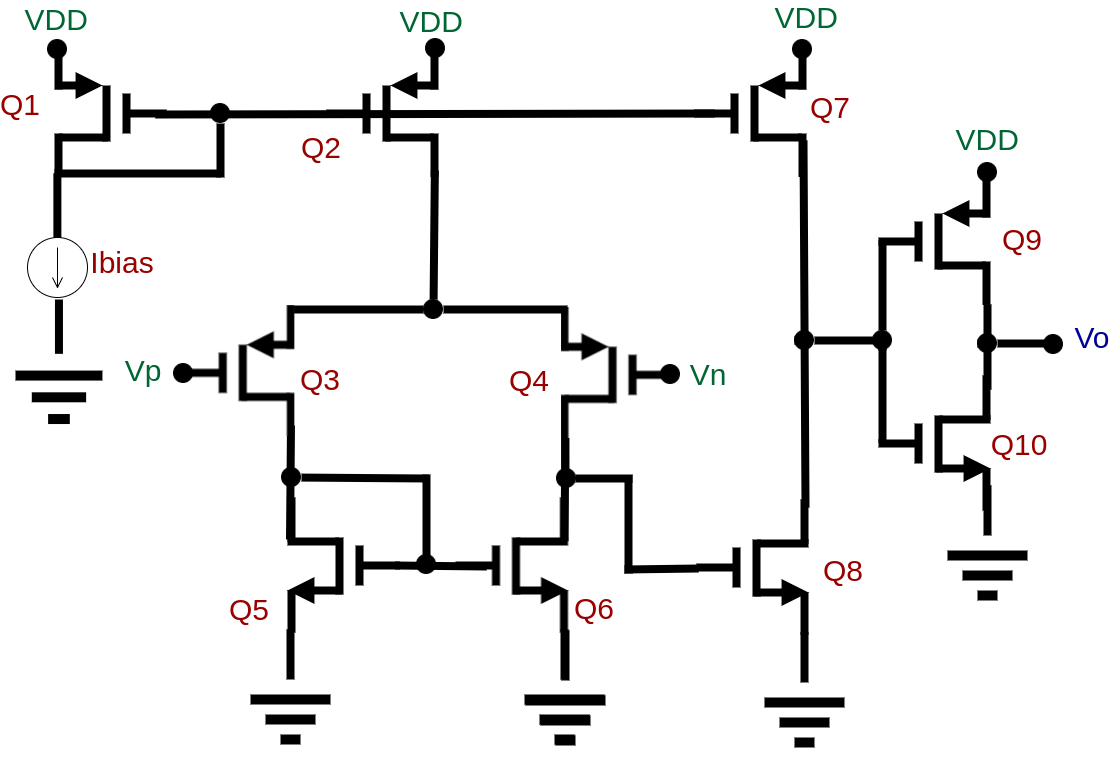
\includegraphics[scale=0.4]{Circuitos/Comparator.png}
    \legend{Fonte: Produzido pelo autor}
\end{figure}

\begin{figure}[htb]
 \centering
    \centering
    \caption{Representa{\c c}\~ao em bloco do \NomeBloco} \label{\NomeSFig}
    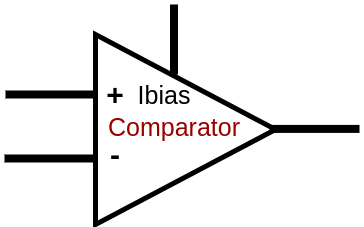
\includegraphics[scale=0.5]{Circuitos/Comparator_block.png}
    \legend{Fonte: Produzido pelo autor}
\end{figure}

Os transistores utilizados no bloco \NomeBloco{} apresentam os par\^ametros mostrados na \autoref{\NomeTTab}.

\begin{table}[htbp]
\caption{Transistores do Bloco \NomeBloco}
\label{\NomeTTab}
\centering
\begin{tabular}{ccccc}
\toprule
Transistor & W ($\mu$m)  & L ($\mu$m)           & M (n° dispositivos) & S (n° dispositivos)\\
\midrule \midrule
Q1 & 10 & 1 & 1 & 1\\
\midrule
Q2$^1$ & 10 & 1 & 6 & 6\\
\midrule
Q3 & 4 & 1 & 2 & 2\\
\midrule
Q4 & 4 & 1 & 2 & 2\\
\midrule
Q5 & 2 & 1 & 2 & 2\\
\midrule
Q6 & 2 & 1 & 2 & 2\\
\midrule
Q7$^1$ & 10 & 1 & 8 & 8\\
\midrule
Q8 & 2 & 1 & 4 & 4\\
\midrule
Q9 & 3 & 0.18 & 1 & 1\\
\midrule
Q10 & 1.5 & 0.18 & 1 & 1\\

\bottomrule
\end{tabular}
\legend{Fonte: Produzido pelo autor}
\legend{$^1$Calculado de forma a produzir uma corrente de 9 $\mu$A}
\end{table}
 
O \NomeBloco{} \'e desenvolvido com tr\^es est\'agios de amplifica{\c c}\~ao. O primeiro est\'agio, composto pelos transistores Q3, Q4, Q5, Q6 t\^em a fun{\c c}\~a de realizar a diferen{\c c}a entra as entradas \emph{Vp} e \emph{Vn} e multiplicar por um pequeno ganho. Os transistores Q3 e Q4 sao respons\'aveis por receber as entradas, enquanto os transistores Q5 e Q6 funcionam como transistores de Carga Ativa. O Q2 funciona como uma fonte de corrente, que ser\'a melhor explicada na \autoref{EspelhoCorrente}.

O segundo est\'agio \'e um est\'agio de ganho, do qual o transistor Q2 fornece um ganho para a saida do est\'agio anterior e o transistor Q7 funciona como uma fonte de corrente para o est\'agio.

O terceiro est\'agio funciona como um amplificador seguidor de fonte, que n\'ao adiciona ganho de tens\~ao por\'em aprimora a resist\'encia de saida do amplificador al\'em de adicionar ganho de corrente.

Diodos quadrados \emph{D1} e \emph{D2} de prote{\c c}\~ao s\~ao inclu\'idos nos terminais \emph{Vp} e \emph{Vn do circuito}, com \^anodo ligado ao terra e catodo ligado ao seu respectivo terminal. Os diodo apresentam os seguintes par\^ametros apresentados na \autoref{diodosComp}.

\begin{table}[htbp]
\caption{Diodos do Bloco \NomeBloco}
\label{diodosComp}
\centering
\begin{tabular}{cccc}
\toprule
Diodo & W ($\mu$m)  & L ($\mu$m)           & \'Area ($\mu$m²)\\
\midrule \midrule
D1 e D2 & 1 & 1 & 1 \\

\bottomrule
\end{tabular}
\legend{Fonte: Produzido pelo autor}
\end{table}
\clearpage